\chapter{Machine learning}
\label{sec:Machine learning}

\section{Supervised learning}
\label{Supervised learning}

%Flow chart
\begin{figure}[H]
\centering
\tikzstyle{largeblock} = [rectangle, draw, fill=blue!20, 
    text width=10em, text centered, rounded corners, minimum height=5em]
\tikzstyle{block} = [rectangle, draw, fill=blue!20, 
    text width=5em, text centered, rounded corners, minimum height=4em]
\tikzstyle{line} = [draw, -latex']
\tikzstyle{cloud} = [draw, ellipse,fill=red!20, node distance=3cm,
    minimum height=2em]
    
\begin{tikzpicture}[node distance = 2.5cm, auto]
    % Place nodes
    \node [cloud] (training) {labeled training data};
    \node [largeblock, below of=training] (machine) {training using machine learning};
    \node [block, right of=machine, node distance=4cm] (classifier) {classifier};
    \node [cloud, right of=training, node distance=4cm] (test) {test data};
    \node [block, below of=classifier] (prediction) {prediction};
    
    
    % Draw edges
    \path [line] (training) -- (machine);
    \path [line] (machine) -- (classifier);
    \path [line] (classifier) -- (prediction);
    \path [line] (test) -- (classifier);

\end{tikzpicture}
\caption{Overview of the system}
\label{system}
\end{figure}


\section{Discrete AdaBoost}
\label{sec:Discret AdaBoost}
For detection of barecodes the machine learning method discrete AdaBoost has been used which is described in \citep{Friedman:2000}. The algorithm is described in \ref{AdaBoost}. The basic idea is to train a number of weak classifiers which during the testing will be combined to a strong classifier. To each data in the training dataset there are corresponding weights which are equal for all data at the beginning. The weak classifiers are trained sequentially and after each step the weights are adjusted depending if they were correctly or incorrectly classified. In each iteration all the training data are used.

\begin{figure} [H]
\line(1,0){250} \newline
Given: $(x_1,y_1),...,(x_m,y_m), \text{where } x_i\in X, y_i \in [-1,+1]$. \newline
$\text{Initialize: } D_1(i)=1/m \text{for } i=1,...,m.$ \newline \newline
$\text{For } t=1,...,T:$
\begin{itemize}
\item $\text{Train weak learner using distribution } D_t.$
\item $\text{Get weak classifier } h_t : X \to {-1,+1}$.
\item \text{Aim: select with low weighted error:}
\begin{center} 

	$\epsilon_t = \sum_{i=1}^{m} D_t(i)I(y_i ! h_t(x_i))$ \newline
	$\text{where I is the split function}$ \newline
\end{center}
\item Chose $ \alpha_t = \frac{1}{2}(\frac{1-\epsilon_t}{\epsilon_t})$
\item Update, for $t = 1,...,m:$
\begin{center} 

	$D_{t+1}(i) = \frac{D_t(i)exp(-\alpha_ty_ih_t(x_i)}{Z_t}$ \newline
	Where $Z_t$ is a normalization factor. \newline
\end{center}
\end{itemize}
Final strong classifier
\begin{center}
	$ H(x) = sign(\sum_{t=1}^{T} {\alpha_th_t(x)}-\varphi)$
\end{center}
\line(1,0){250}
\caption{Algorithm for discrete AdaBoost}
\label{AdaBoost}
\end{figure}


The split functions may consist of a number of different parameters. The most basic function, which has been used here, only has one parameter, a threshold. The function search for a threshold in one dimension at a time and choose the one which best separates the data.

\section{Discrete Random forest}
\label{sec:Discret Random forest}
Random forest is described in \citep{Criministi:2011}. The algorithm creates decision trees which in the end are combined to a strong classifier. For each tree only a randomly chosen subset of the training data is used. This is in contrast to the AdaBoost algorithm where all training data are used in each iteration. The Ranom forest can be used for classification with more than two classes which is one of the advantage to AdaBoost. This makes it a lot more suitable for character recognition.

During training the trees are created one at a time with a random subset of training data. In each split node in a tree it is possible to use the whole feature vector or just a part of it. This depends on the amount of features. For a problem with a large amount of features it is common to chose a specific number of features randomly for every split.  

\begin{figure}[H]
\centering
	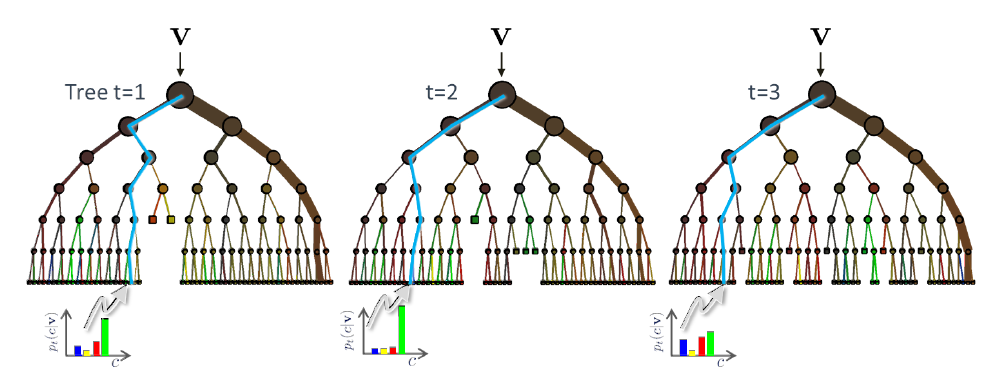
\includegraphics[scale=0.5]{RandomForest}
	\caption{Image illustrates testing using Random forest. Source: \citep{Criministri:2011}}
	\label{randomforest}
\end{figure}
 
% Local Variables:
% TeX-master: "main.tex"
% End:
